\documentclass{article}%
\usepackage[T1]{fontenc}%
\usepackage[utf8]{inputenc}%
\usepackage{lmodern}%
\usepackage{textcomp}%
\usepackage{lastpage}%
\usepackage[head=40pt,margin=0.5in,bottom=0.6in]{geometry}%
\usepackage{graphicx}%
%
\title{\textbf{Misión de la OEA vio en la frontera el desespero de familias venezolanas}}%
\author{GDA | EL TIEMPO | COLOMBIA | EFE}%
\date{21/11/2018}%
%
\begin{document}%
\normalsize%
\maketitle%
\textbf{URL: }%
http://www.el{-}nacional.com/noticias/mundo/mision{-}oea{-}vio{-}frontera{-}desespero{-}familias{-}venezolanas\_260523\newline%
%
\textbf{Periodico: }%
EN, %
ID: %
260523, %
Seccion: %
Mundo\newline%
%
\textbf{Palabras Claves: }%
NO\_TIENE\newline%
%
\textbf{Derecho: }%
18%
, Otros Derechos: %
NO\_TIENE%
, Sub Derechos: %
NO\_TIENE%
\newline%
%
\textbf{EP: }%
NO\newline%
\newline%
%
\textbf{\textit{Luego de recorrer el lunes zonas de La Guajira y Norte de Santander, la misión diplomática describió como muy triste la situación de los migrantes}}%
\newline%
\newline%
%
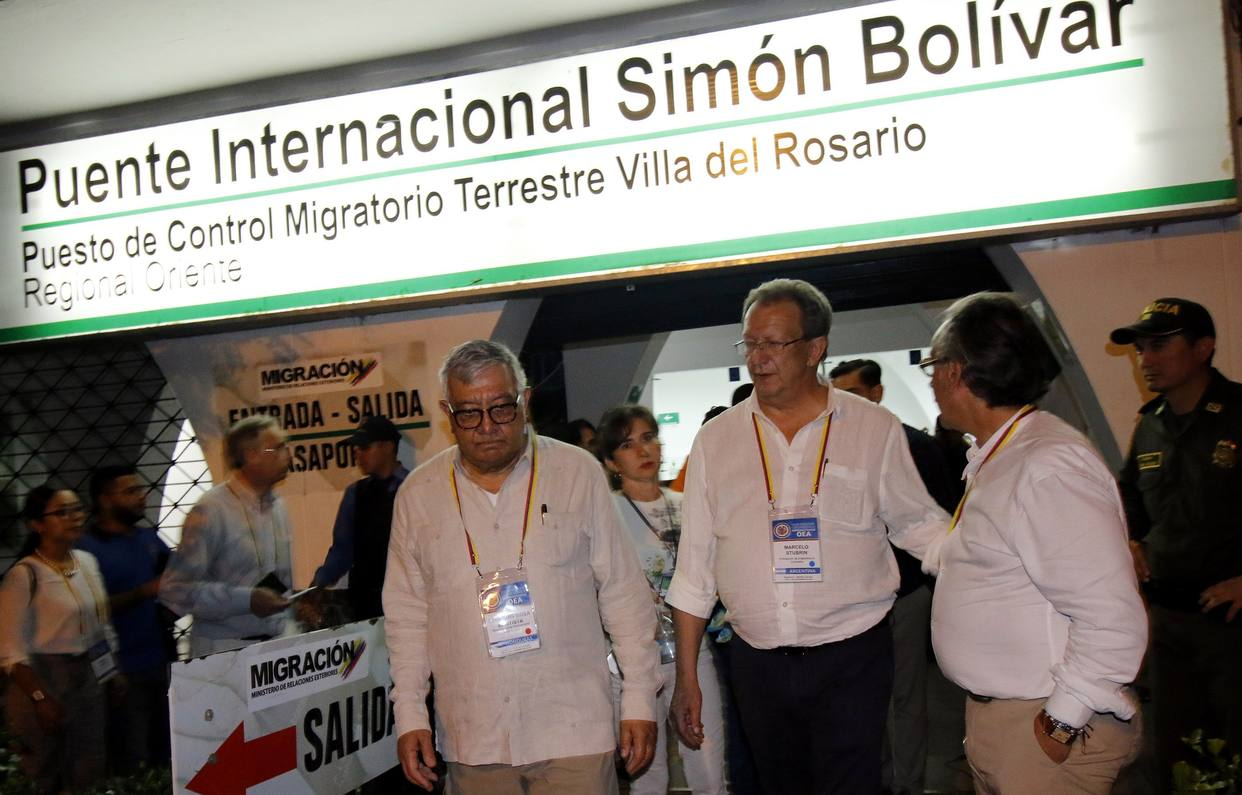
\includegraphics[width=300px]{160.jpg}%
\newline%
%
Tras visitar los departamentos de~La Guajira~y Norte de Santander, una comisión integrada por 17 países miembros de~la OEA~reiteró la necesidad de plantear una solución pacífica a la crisis venezolana, que ha desatado una ola migratoria sin precedentes.%
\newline%
%
La delegación inició su recorrido en Maicao y Paraguachón (La Guajira), y en la tarde se trasladó a Cúcuta.~En la capital nortesatandereana ~los embajadores mantuvieron un encuentro con las autoridades y aprovecharon para insistir en una solución pacífica a la debacle del gobierno de Venezuela.~“Hemos visto con nuestros ojos lo que está sucediendo: la cara de niños, mujeres y padres, saliendo desesperados por cruzar una frontera con valijas vacías solo para retornar con un poco de alimento y sobrevivir.~Es algo muy triste, que desde~la OEA~estamos buscando una solución pacífica para cumplir”, indicó Carlos Trujillo, embajador de Estados Unidos ante ese organismo internacional.de la visita diplomática, liderada por Argentina, Belice, Chile, Costa Rica, Colombia, Ecuador, Estados Unidos, Guatemala, Guyana, Haití, Honduras, Jamaica, Panamá, Paraguay, Perú, Santa Lucía y Uruguay,~se elaborará un informe con el fin de propender medidas de la comunidad internacional para encarar desde varios frentes el flujo de migrantes.%
\newline%
%
El gobernador de Norte de Santander, William Villamizar Laguado, pidió que esa visita no se redujera a un simple periplo internacional, sino que se tradujera en alternativas para afrontar el fenómeno.“Esta es la manera de tratar una problemática como la que estamos viviendo en el departamento.~Esperamos que las ayudas lleguen a través de recursos o de una presión de un gobierno para que logre buscar las soluciones sin ocasionar problemas a otros países”, dijo el funcionario.%
\newline%
%
Sanciones severas.~En declaraciones al diario~El Observador, el secretario general de~la OEA, Luis Almagro, señaló que muchos venezolanos fueron expulsados del país a través del hambre o de la persecución política, por lo que han puesto a disposición todas las herramientas para cooperar con Venezuela. “Hemos hecho lo que deberíamos hacer. Sanciones cada vez más fuertes, que afecten al gobierno, a la dictadura, y que definitivamente le tuerzan el brazo para una solución institucional que el país necesita”.%
\newline%
%
MEDIDA%
\newline%
%
Expulsan a 15 migrantes por desmanes%
\newline%
%
Las autoridades de Colombia expulsaron a 15 venezolanos que participaron en los desmanes en el campamento al que fueron trasladados más de 400 ciudadanos que huyen de la crisis en el país, informaron fuentes oficiales.%
\newline%
%
Los expulsados forman parte de un grupo de más de 400 venezolanos que la semana pasada fueron reubicados por~la Alcaldía~de Bogotá en Engativá. El lunes se involucraron graves disturbios al saquear alacenas, enfrenarse a la policía e incluso agredir a ~habitantes de la zona.%
\newline%
%
Los inmigrantes protestaban porque, según ellos, la calidad de la comida que les suministran es mala, poca y hasta vencida. Asimismo, porque no les permiten ingresar donaciones de alimentos.%
\newline%
%
El director de Migración Colombia, Christian Krüger, dijo que la idea del campamento fue la de mejorar las condiciones de vida de esas personas, pero que no ~permitirán comportamientos que pongan en riesgo la integridad de la población colombiana e incluso de la que se encuentra en el campamento.%
\newline%
%
\end{document}